\documentclass[11pt]{article}
\usepackage{graphicx}
\usepackage{amssymb}
\usepackage{epstopdf}
\usepackage[usenames]{color}
\usepackage{psfrag}
\usepackage{textcomp}
\usepackage{wrapfig}

%\DeclareGraphicsRule{.tif}{png}{.png}{`convert #1 `dirname #1`/`basename #1 .tif`.png}

\textwidth = 6.5 in
\textheight = 9 in
\oddsidemargin = 0.0 in
\evensidemargin = 0.0 in
\topmargin = 0.0 in
\headheight = 0.0 in
\headsep = 0.0 in
\parskip = 0.2in
\parindent = 0.0in

\newcommand\Ro{\mbox{\textrm Ro}}
\newcommand\Ra{\mbox{\textrm Ra}}
\newcommand\Nu{\mbox{\textrm Nu}}
\newcommand\Rey{\mbox{\textrm Re}}
\newcommand\Pran{\mbox{\textrm Pr}}

\newcommand\remark[1]{{\footnotesize \color{green}Comment: #1}}

\graphicspath{{./Figures/}}

\begin{document}
\section{Calculating the real heat conduction}
Here, we test various assumptions made by \cite{SU15}.
First, we see, whether the assumption of an effective temperature difference holds:
\[
\Delta_{eff} = 2(T_b-T_c)\mbox{,}
\]

For this test, we calculate the real heat conduction $q_{cond}$ based on the heat conduction at every point
$\lambda(z)$ and integrating the:
\[
q_{cond} = \lambda(z) \frac{\partial T}{\partial z}\mbox{.}
\]

The integration is done via a shooting method starting from the top plate temperature $T_t$ with a varying
parameter $q_{cond}$ to hit $T_b$ at z=L (L being the height). 

From the real temperature profile T(z) one calculates the density $\varrho$ at each z and subsequently the
hydrostatic pressure p(z) $\partial p /\partial z = g\varrho z$. In this integration, there is a constant $p_0$
that is chosen such that $p(L/2) = P_m$ being the pressure in the U-Boot. From p(z) and T(z) we recalculate
the fluid properties $\varrho(z)$ and $\lambda(z)$, that we plug back into Ficks law. In an iterative way, we
get the real profile $T(z)$, p(z), $\varrho(z)$, and $\alpha(z)$.

For test purposes, I assume: L=2.2m;$T_b=40$C; $T_t=13$C and P=19\,bar. We note, that $T_t$ at this pressure
is already in the liquid regime. However, the SF6 program (by Guenter) extrapolate the gas values into this
regime. For test purposes this should be fine.

Integration is done with 10000 intervals (in z-direction) using a simple Euler scheme.

Already after 2 iterations, q has reached its final value:
Iteration:
\begin{itemize}
 \item 	0: q = 0.189488 [W/m$^2$] (linear profile)
 \item 	1: q = 0.190150 [W/m$^2$]
 \item 	 :
 \item 	6: q = 0.190202 [W/m$^2$] 
 \item Heat conduction assuming linear profile and $\lambda(T_m)$: $q_{cond}= 0.1895 W/m^2$
\end{itemize}

\begin{figure}[htpb]
\centering
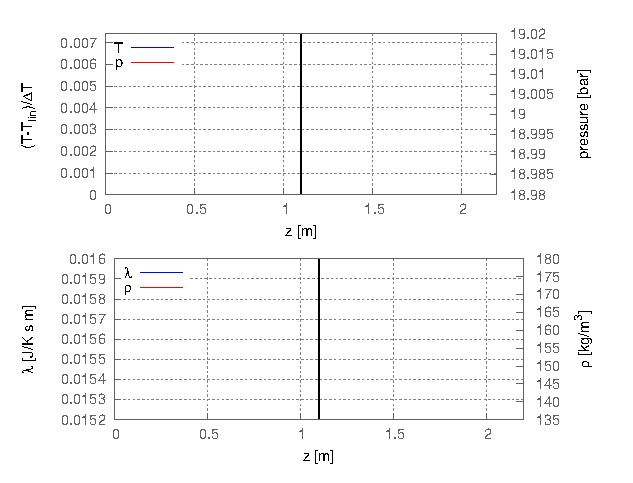
\includegraphics[width=\textwidth]{Fig/6th_Iter.eps}
\caption{Top: Variation from the linear Temperature profile and pressure profile p(z).
Bottom: Density $\varrho(z)$ and heat heat conductivity $\lambda(z)$. {\bf Note, that the z- axis shows in downward
direction (against usual convention).} The vertical black line shows the midheight of the cell.}
\label{fig:Iter}
\end{figure}

The result shows, that in this regime the conductive heat transport $q_{cond}$ can well be approximated by
$q_{cond}\approx \lambda (T_m)\Delta T/L$. The reason becomes clear from fig.~\ref{fig:Iter}. The variation of
the temperature from a linear profile is small in comparision to $\Delta T$. The hydrostatic pressure is
rather small and thus also $\lambda$ doesn't change significant with z. Only $\varrho$ changes remarkable due
to the temperature gradients.

\begin{figure}[htpb]
\centering
\includegraphics[width=\textwidth]{Fig/alpha.eps}
\caption{The normalised heat expansion coefficient as a function of z, assuming the T(z) and p(z) as shown in
fig.~\ref{fig:Iter}. The vertical black line shows the midheight of the cell.}
\label{fig:alpha}
\end{figure}

\section{Analysing $\Gamma=1$-Data}

In the following, we analyse the $\Gamma=1$- data, provided by Xiaozhou.
As we have seen above, $q_{cond}$ doesn't change much when numerically calculated versus via
$\lambda(T_m)\Delta T/L$.

We use in the following: L=1.12\,m. The result of an reanalysis is shown in fig.~\ref{fig:Ra_Nu}. One clearly
sees that whatever $q_{cond}$ we choose, the differences in $Nu/Ra^{1/3}$ is small. In particular, the
transition at around $Ra=10^{14}$ is clearly visible. However, any corrections reduces $Nu/Ra^{1/3}$ slightly.
The blue bullets show the original analysis with fluid properties evaluated at $T_m=(T_t+T_b)/2$. Using the
numerically calculated conduction profile for calculating Nu (denoted as $Nu_r$) decreases Nu very little
(less than 0.2\%). The largest degrease is visible in the open pink squares, that show the numerically
calculated Nu, normalised by $Ra_c$ which is Ra with the fluid parameters calculated at the midheight
temperature $T_c$.

\begin{figure}[htpb]
\centering
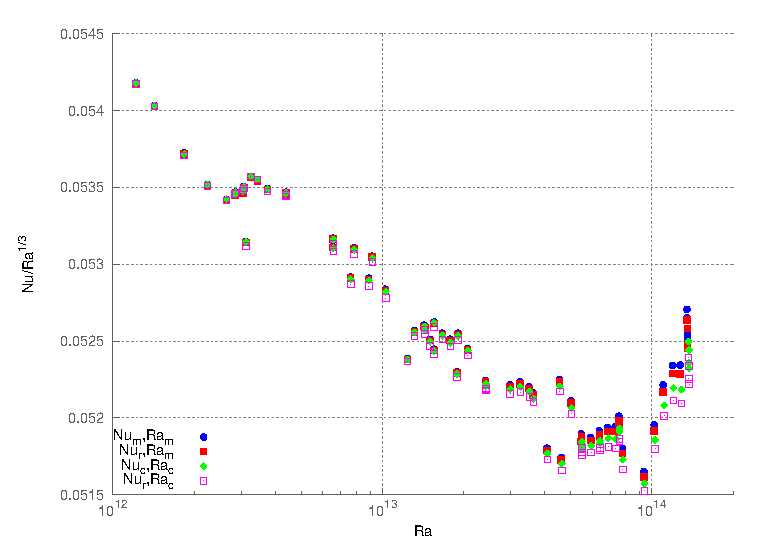
\includegraphics[width=\textwidth]{Ra_Nu.eps}
\caption{Various ways to calculate Nu and Ra compared with each other. Data are from the
$\Gamma=1$-experiment. $Nu_r$ denote Nu based on the real numerically calculated $q_{cond}$. $Nu_m$ stands for
Nu with $q_{cond}$ calculated $\lambda(T_m)$, and $Nu_c$ uses $\lambda(T_c)$. Similarly for Ra.}
\label{fig:Ra_Nu}
\end{figure}


\bibliographystyle{unsrt}
\bibliography{/home/stevie/ownCloud/Literature/bibliography}

\end{document} 
